\chapter{Photosynthesis}\label{photosynthesis}

In this lab, we will study the effect of light intensity and quality
(wave length - color) on
\href{https://en.wikipedia.org/wiki/Photosynthesis}{photosynthesis}. As
a measure of the rate of photosynthesis, we will monitor the rate of
oxygen production. When plants that spend their life submerged in water
release oxygen it forms bubbles, which we can count over a period of
time to determine photosynthesis rate.

Photosynthesis is a process used by plants and other organisms to
convert light energy into chemical energy that can later be released to
fuel the organisms' activities (energy transformation). This chemical
energy is stored in carbohydrate molecules, such as sugars, which are
synthesized from carbon dioxide and water - hence the name
photosynthesis, from the Greek phōs, ``light'', and synthesis, ``putting
together''. In most cases, oxygen is also released as a waste product.
Most plants, most algae, and cyanobacteria perform photosynthesis; such
organisms are called photoautotrophs. Photosynthesis is largely
responsible for producing and maintaining the oxygen content of the
Earth's atmosphere, and supplies all of the organic compounds and most
of the energy necessary for life on Earth.

Although photosynthesis is performed differently by different species,
the process always begins when energy from light is absorbed by proteins
called reaction centers that contain green chlorophyll pigments. In
plants, these proteins are held inside organelles called chloroplasts,
which are most abundant in leaf cells, while in bacteria they are
embedded in the plasma membrane. In these light-dependent reactions,
some energy is used to strip electrons from suitable substances, such as
water, producing oxygen gas. The hydrogen freed by the splitting of
water is used in the creation of two further compounds that act as an
immediate energy storage means: reduced nicotinamide adenine
dinucleotide phosphate (NADPH) and adenosine triphosphate (ATP), the
``energy currency'' of cells.

In plants, algae and cyanobacteria, long-term energy storage in the form
of sugars is produced by a subsequent sequence of light-independent
reactions called the Calvin cycle; some bacteria use different
mechanisms, such as the reverse Krebs cycle, to achieve the same end. In
the Calvin cycle, atmospheric carbon dioxide is incorporated into
already existing organic carbon compounds, such as ribulose bisphosphate
(RuBP). Using the ATP and NADPH produced by the light-dependent
reactions, the resulting compounds are then reduced and removed to form
further carbohydrates, such as glucose.

The first photosynthetic organisms probably evolved early in the
evolutionary history of life and most likely used reducing agents such
as hydrogen or hydrogen sulfide, rather than water, as sources of
electrons. Cyanobacteria appeared later; the excess oxygen they produced
contributed directly to the oxygenation of the Earth, which rendered the
evolution of complex life possible. Today, the average rate of energy
capture by photosynthesis globally is approximately 130 terawatts which
is about three times the current power consumption of human
civilization. Photosynthetic organisms also convert around 100-115
thousand million metric tons of carbon into biomass per year.

The main source of light on Earth is the Sun. Sunlight provides the
energy that green plants use to create sugars mostly in the form of
starches, which release energy into the living things that digest them.
This process of photosynthesis provides virtually all the energy used by
living things. The primary properties of visible light are intensity,
propagation direction, frequency or wavelength spectrum, and
polarization, while its speed in a vacuum, 299,792,458 meters per
second, is one of the fundamental constants of nature. Visible light, as
with all types of electromagnetic radiation (EMR), is experimentally
found to always move at this speed in a vacuum.

\section{Intensity of light}\label{intensity-of-light}

\href{https://en.wikipedia.org/wiki/Light}{Light} is electromagnetic
radiation within a certain portion of the electromagnetic spectrum
(Figure \ref{fig:spectrum}). The word usually refers to visible light,
which is visible to the human eye and is responsible for the sense of
sight. Visible light is usually defined as having wavelengths in the
range of 400-700 nanometres (nm), or 400 × 10\textsuperscript{-9} to 700
× 10\textsuperscript{-9} m, between the infrared (with longer
wavelengths) and the ultraviolet (with shorter wavelengths). This
wavelength means a frequency range of roughly 430-750 terahertz (THz).

\begin{figure}

{\centering 
\includegraphics[width=0.7\linewidth]{./figures/photosynthesis/spectrum}

}

\caption{\href{https://commons.wikimedia.org/wiki/File:Linear_visible_spectrum.svg}{Spectrum
of light. V, violet; B, blue; G, green Y, yellow; O, orange; R, red}}\label{fig:spectrum}
\end{figure}

In this experiment (Figure \ref{fig:photosynthesis}), we will study the
effect of light intensity on the photosynthetic activity of \emph{Elodea
canadensis}. We will vary the light intensity by changing the distance
between the light source and the plant. We will count the emerging
oxygen bubbles as an indicator of the photosynthetic activity of the
plant.

\begin{figure}

{\centering 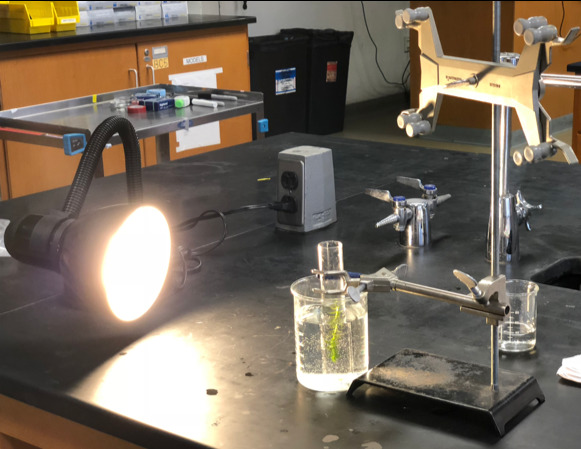
\includegraphics[width=0.7\linewidth]{./figures/photosynthesis/photosynthesis}

}

\caption{Setup for photosynthesis experiment.}\label{fig:photosynthesis}
\end{figure}

\subsection{Experimental procedures}\label{experimental-procedures-21}

\begin{enumerate}
\def\labelenumi{\arabic{enumi}.}
\tightlist
\item
  Select a fresh, crisp sprig of Elodea about 15 cm in length.
\item
  While the plant is still submerged, cut 2-3 mm from its base.
\item
  Place the sprig upside down in a test tube filled with 0.3\% sodium
  bicarbonate. This is a buffer to absorb toxic materials evolved (i.e.,
  that are released. Keeping the plant submerged, position a light
  source 1 foot away and adjust so the light shines directly on the
  plant.
\item
  Place the test tube in a beaker of water as shown in Fig.
  \ref{fig:photosynthesis} to prevent overheating the plant. Allow the
  system to stand 7-10 minutes, or until bubbles begin to appear
  regularly.
\item
  Count the bubbles produced each minute for a 5-minute period and
  average them. Record your findings in the table.
\item
  Move the light back 2 feet from the plant, wait 5 minutes, and repeat
  counting. Record your findings in Table \ref{tab:intensity}.
\item
  Move the light back to 3 feet from the plant and repeat counting the
  bubbles.
\end{enumerate}

\begin{longtable}[]{@{}llllllc@{}}
\caption{\label{tab:intensity} Intensity of light.}\tabularnewline
\toprule
Distance of light source/Bubbles per minute & 1 & 2 & 3 & 4 & 5 &
Average\tabularnewline
\midrule
\endfirsthead
\toprule
Distance of light source/Bubbles per minute & 1 & 2 & 3 & 4 & 5 &
Average\tabularnewline
\midrule
\endhead
1 foot & & & & & &\tabularnewline
2 feet & & & & & &\tabularnewline
3 feet & & & & & &\tabularnewline
\bottomrule
\end{longtable}

\begin{figure}

{\centering 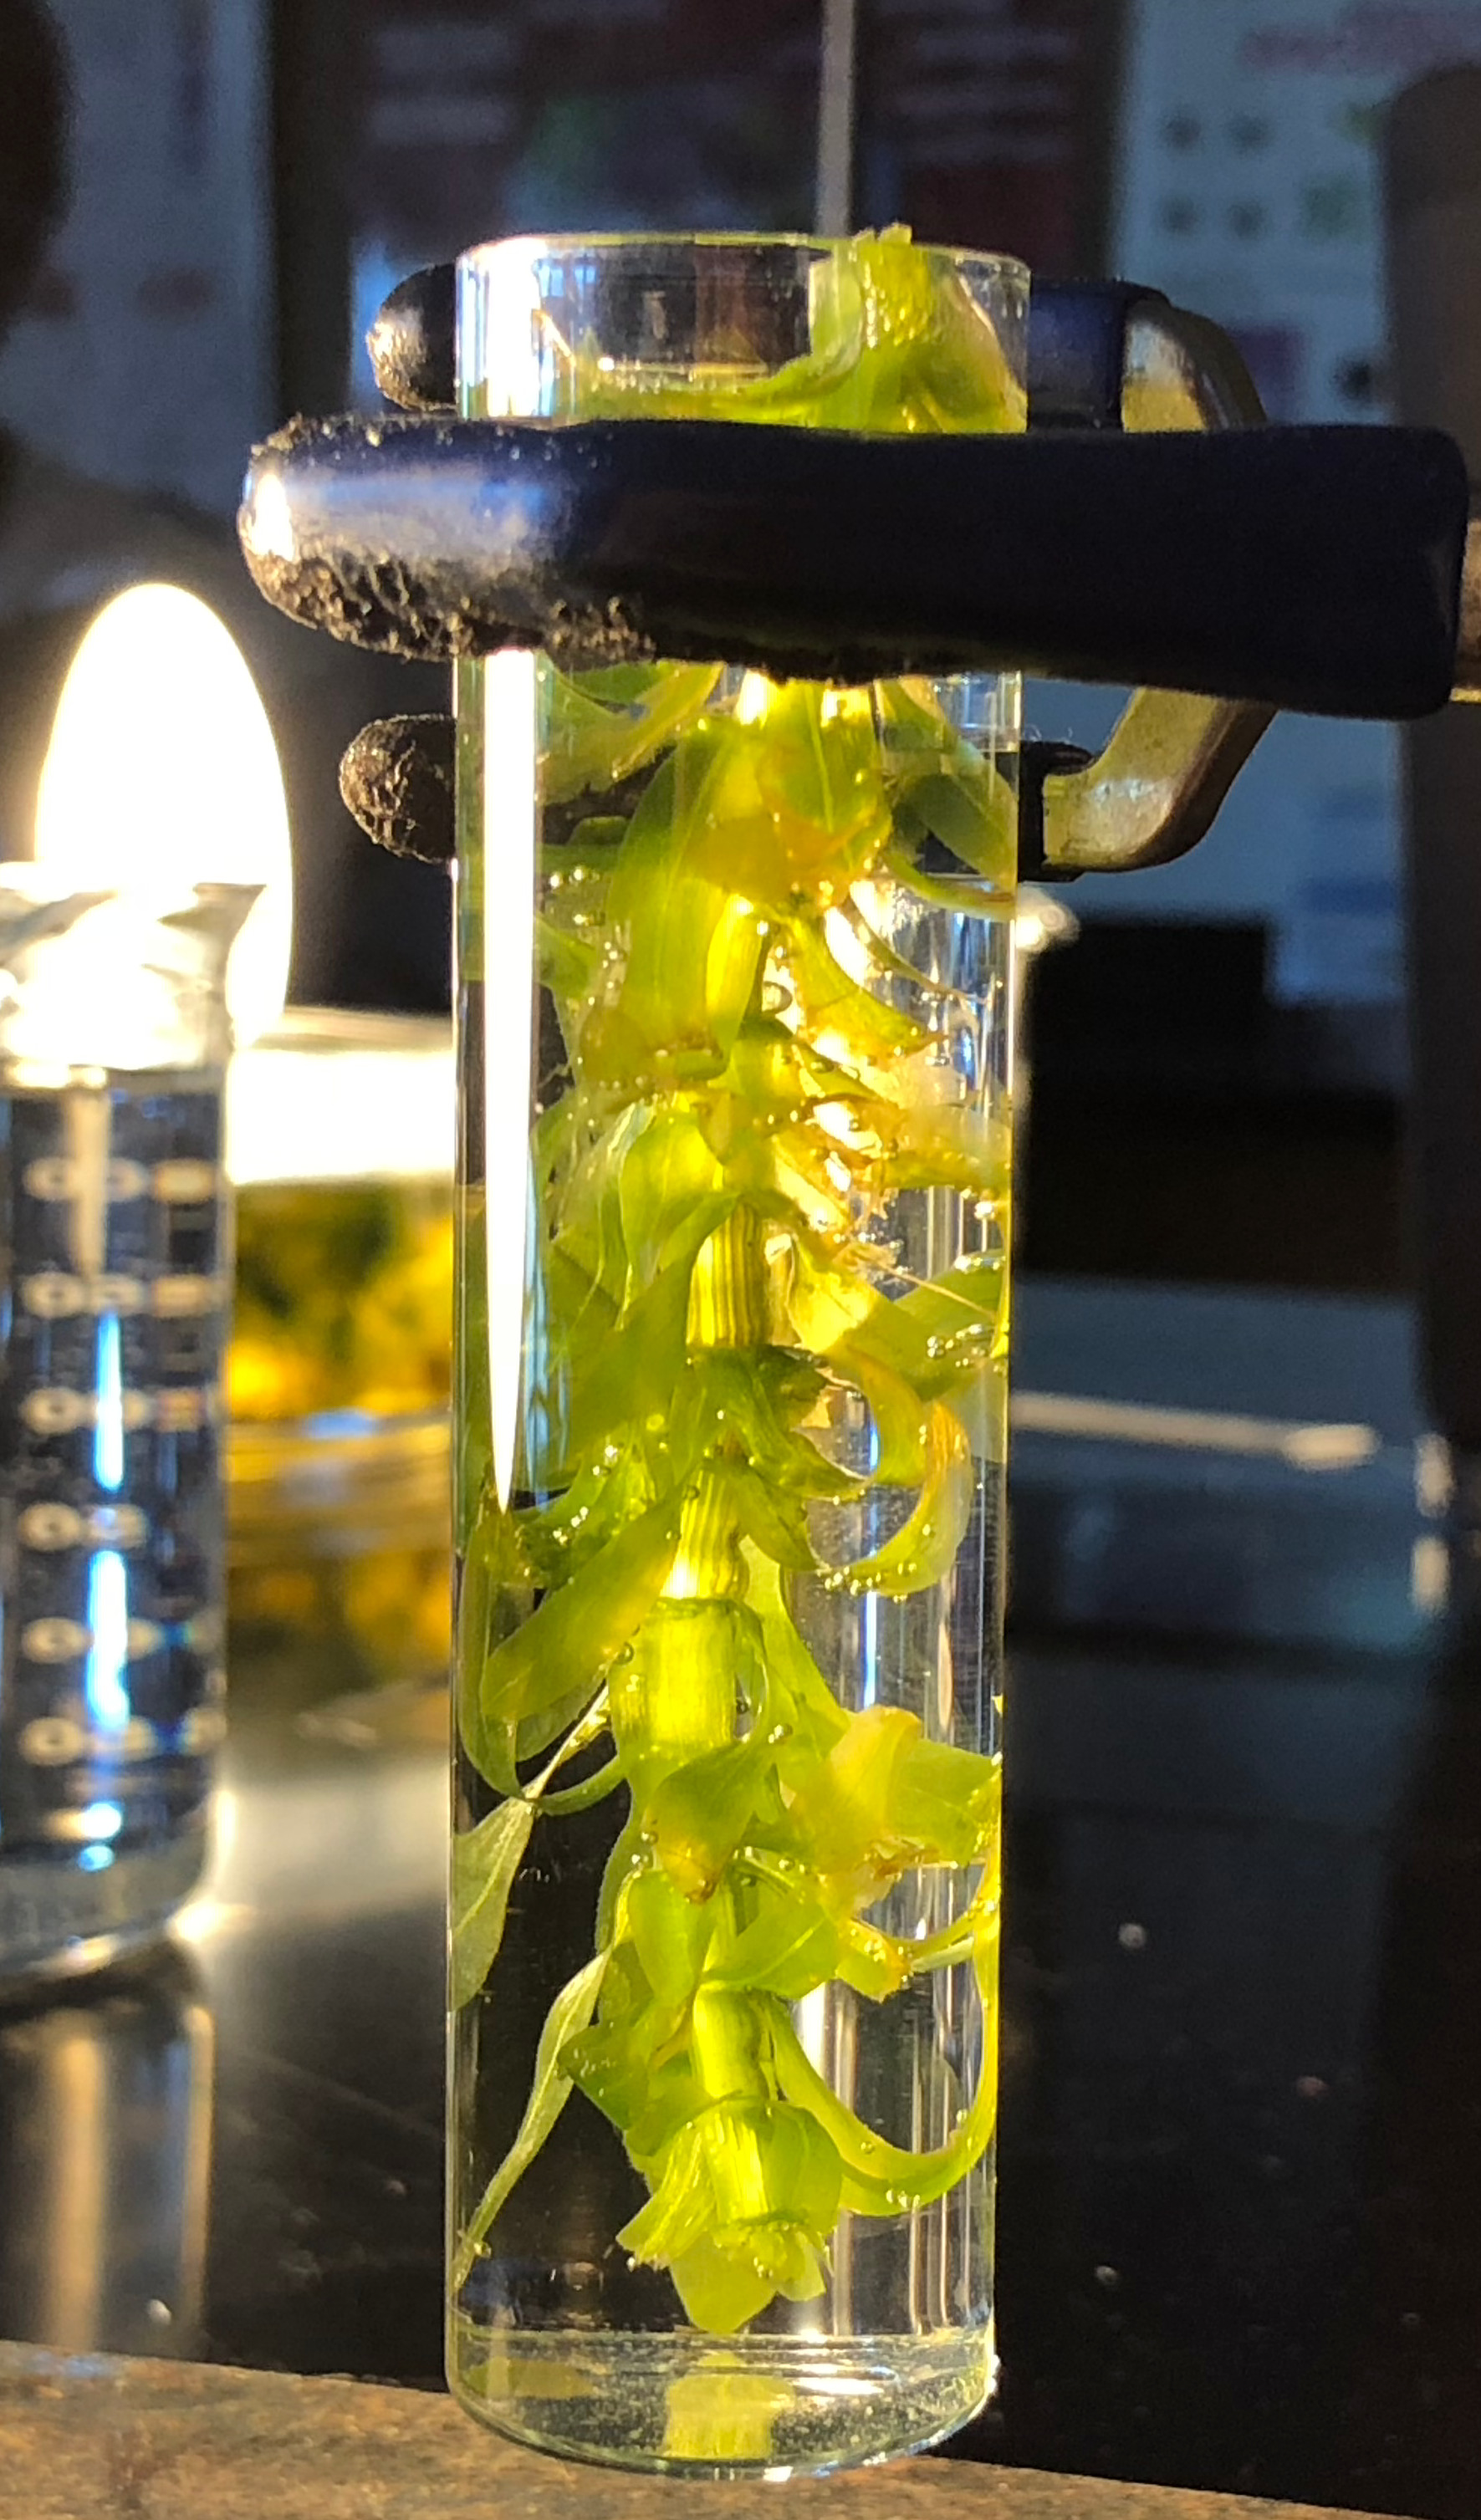
\includegraphics[width=0.7\linewidth]{./figures/photosynthesis/photosynthesis_bubbles}

}

\caption{Appearance of bubbles indicates active photosynthesis.}\label{fig:bubbles}
\end{figure}

\section{Color of light}\label{color-of-light}

In this experiment, we will study the effect of the color of light on
the photosynthetic activity of \emph{Elodea canadensis}. We will use
filter to expose the plant to light of only a limited range of
wavelengths. We will again count the emerging oxygen bubbles as an
indicator of the photosynthetic activity of the plant.

\subsection{Experimental procedures}\label{experimental-procedures-22}

\begin{enumerate}
\def\labelenumi{\arabic{enumi}.}
\tightlist
\item
  Select a fresh, crisp sprig of Elodea about 15 cm in length.
\item
  While the plant is still submerged, cut 2-3 mm from its base.
\item
  Place the sprig upside down in a test tube filled with 0.3\% sodium
  bicarbonate. This is a buffer to absorb toxic materials evolved (i.e.,
  that are released). Keeping the plant submerged, position a light
  source 1 foot away and adjust so the light shines directly on the
  plant.
\item
  Place a colored filter between the test tube and the heat shield
  beaker and allow it to sit for 5 minutes.
\item
  Count bubbles for 5 minutes as in the previous experiment. Record your
  findings in Table \ref{tab:color}. Repeat steps 1 and 2 for each color
  filter available.
\end{enumerate}

\begin{longtable}[]{@{}llllllc@{}}
\caption{\label{tab:color} Color of light.}\tabularnewline
\toprule
Color of filter/Bubbles per minute & 1 & 2 & 3 & 4 & 5 &
Average\tabularnewline
\midrule
\endfirsthead
\toprule
Color of filter/Bubbles per minute & 1 & 2 & 3 & 4 & 5 &
Average\tabularnewline
\midrule
\endhead
blue & & & & & &\tabularnewline
orange & & & & & &\tabularnewline
red & & & & & &\tabularnewline
\bottomrule
\end{longtable}

\section{Determination of the light absorption spectrum of dye
solutions}\label{determination-of-the-light-absorption-spectrum-of-dye-solutions}

In this experiment, we will use a
\href{https://en.wikipedia.org/wiki/Spectrophotometry}{spectrophotometer}
to measure the differential absorption of light of different wavelength
by water stained with food dyes.

\begin{figure}

{\centering 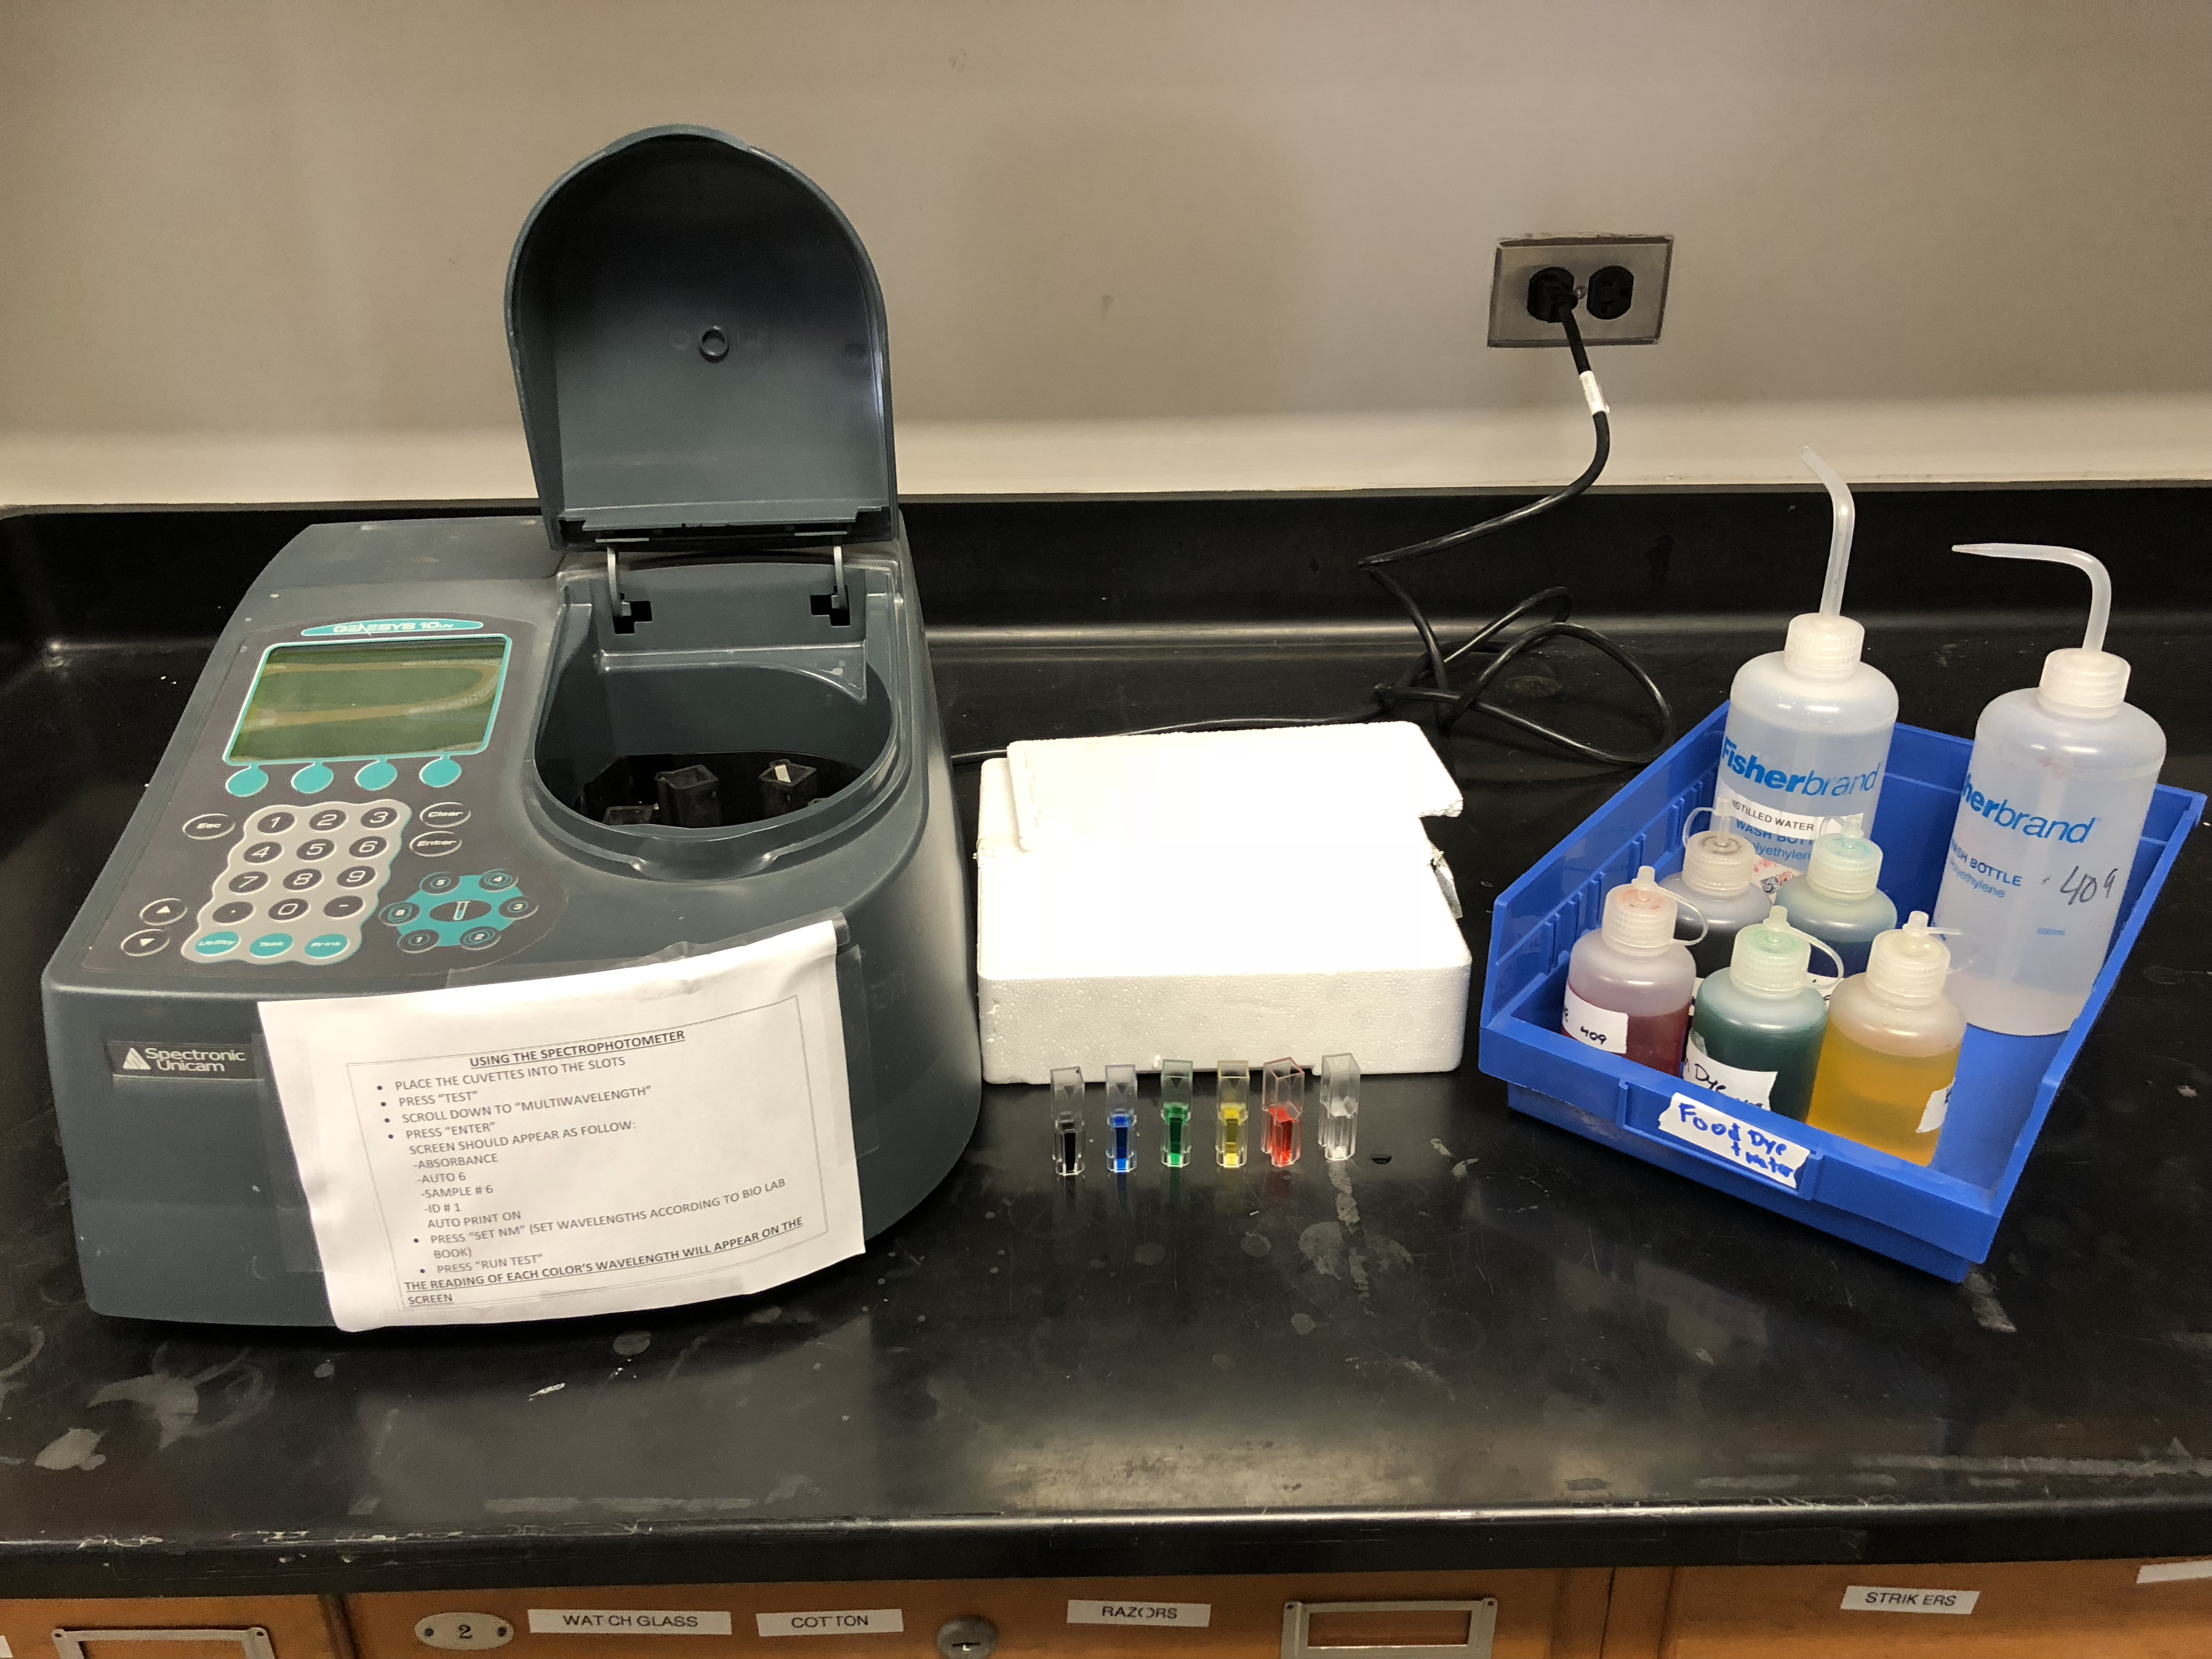
\includegraphics[width=0.7\linewidth]{./figures/photosynthesis/spectrophotometer}

}

\caption{Spectrophotometer and cuvettes with dye solutions.}\label{fig:spectrophotometer}
\end{figure}

\subsection{Experimental procedures}\label{experimental-procedures-23}

\begin{enumerate}
\def\labelenumi{\arabic{enumi}.}
\tightlist
\item
  Take six cuvettes.
\item
  Fill one cuvette with water.
\item
  Fill each of the remaining five cuvettes with one of the color
  solutions listed in Table \ref{tab:absorption}.
\item
  Insert the cuvette with water into the slot marked ``B''.
\item
  Insert the other cuvettes into the slots marked 1 to 5 and write down
  which color is in which slot.
\item
  Following the instructions posted on the spectrophotometer, program
  the machine to take absorption measurements at wavelengths between
  380-740 nm in 20 nm steps.
\item
  Once the measurements are completed, write down the absorption number
  for each dye and wavelength.
\item
  Use a spreadsheet program to graph your results.
\item
  Compare your curves with the data shown in Figure
   \ref{fig:absorption}.
\end{enumerate}

\begin{figure}

{\centering 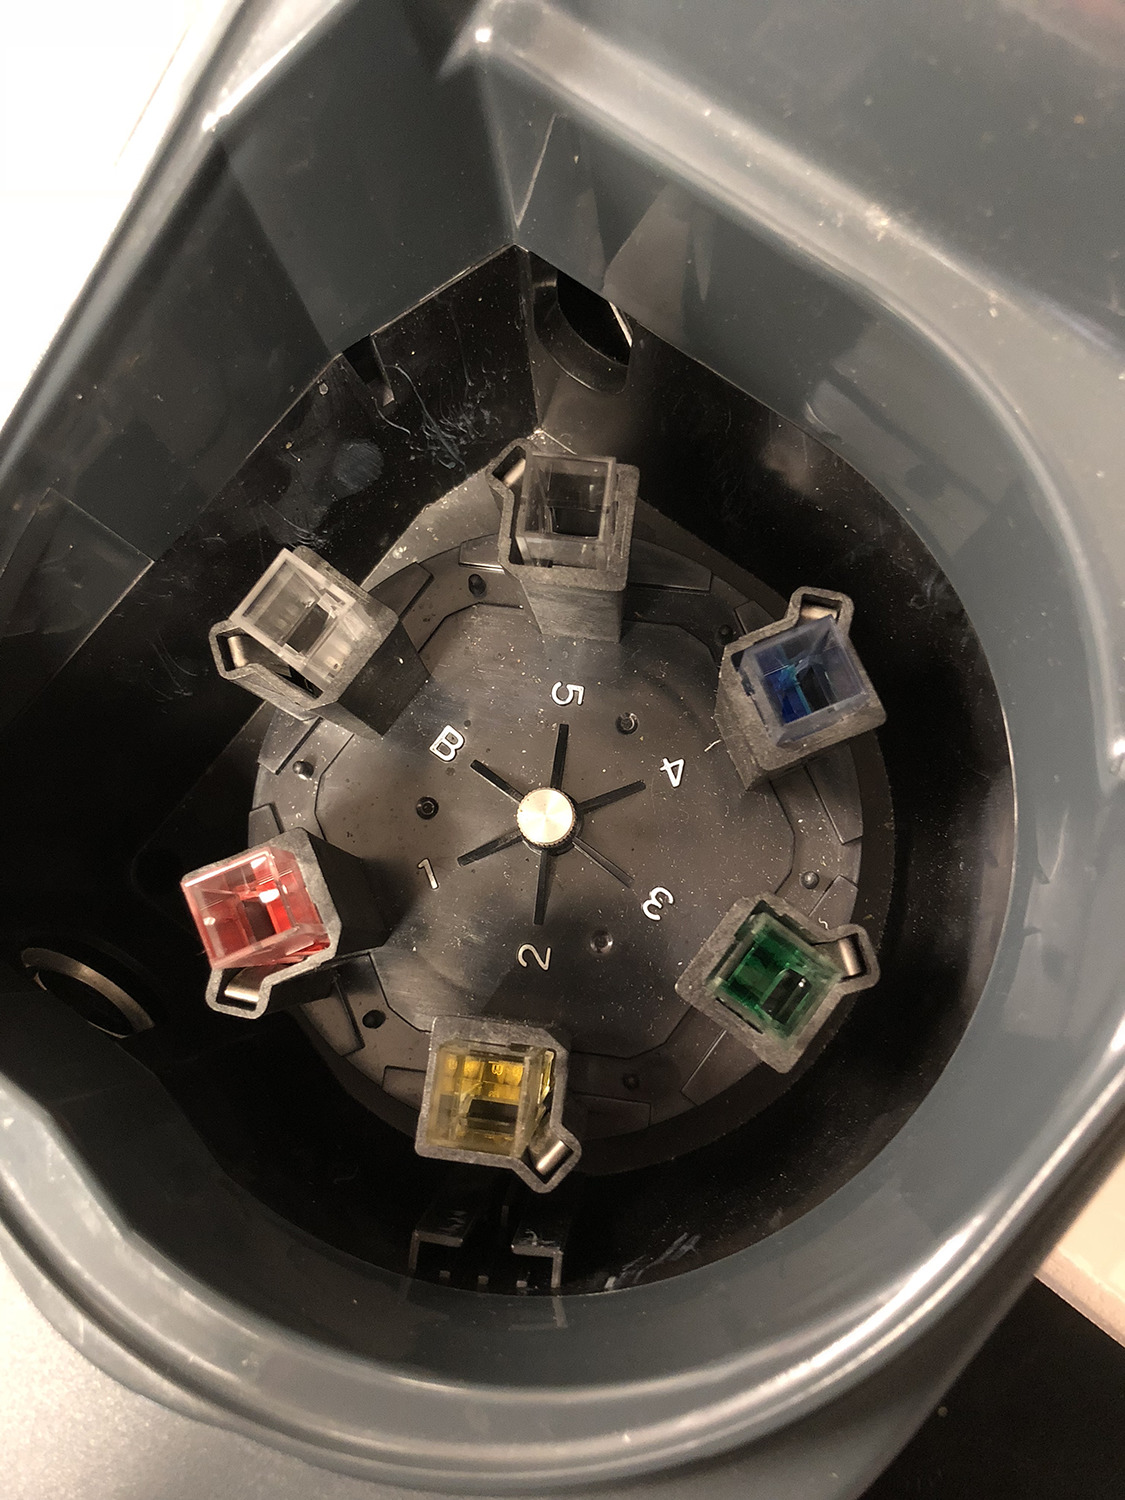
\includegraphics[width=0.7\linewidth]{./figures/photosynthesis/cuvettes}

}

\caption{Cuvettes placed in the spectrophotometer.}\label{fig:cuvettes}
\end{figure}

\begin{longtable}[]{@{}clllll@{}}
\caption{(\label{tab:absorption} Determination of the light absorption
spectrum of dye solutions.}\tabularnewline
\toprule
Wavelength (nm) & Purple & Blue & Green & Yellow & Red\tabularnewline
\midrule
\endfirsthead
\toprule
Wavelength (nm) & Purple & Blue & Green & Yellow & Red\tabularnewline
\midrule
\endhead
380 & & & & &\tabularnewline
400 & & & & &\tabularnewline
420 & & & & &\tabularnewline
\ldots{} & & & & &\tabularnewline
720 & & & & &\tabularnewline
740 & & & & &\tabularnewline
\bottomrule
\end{longtable}

\begin{figure}

{\centering 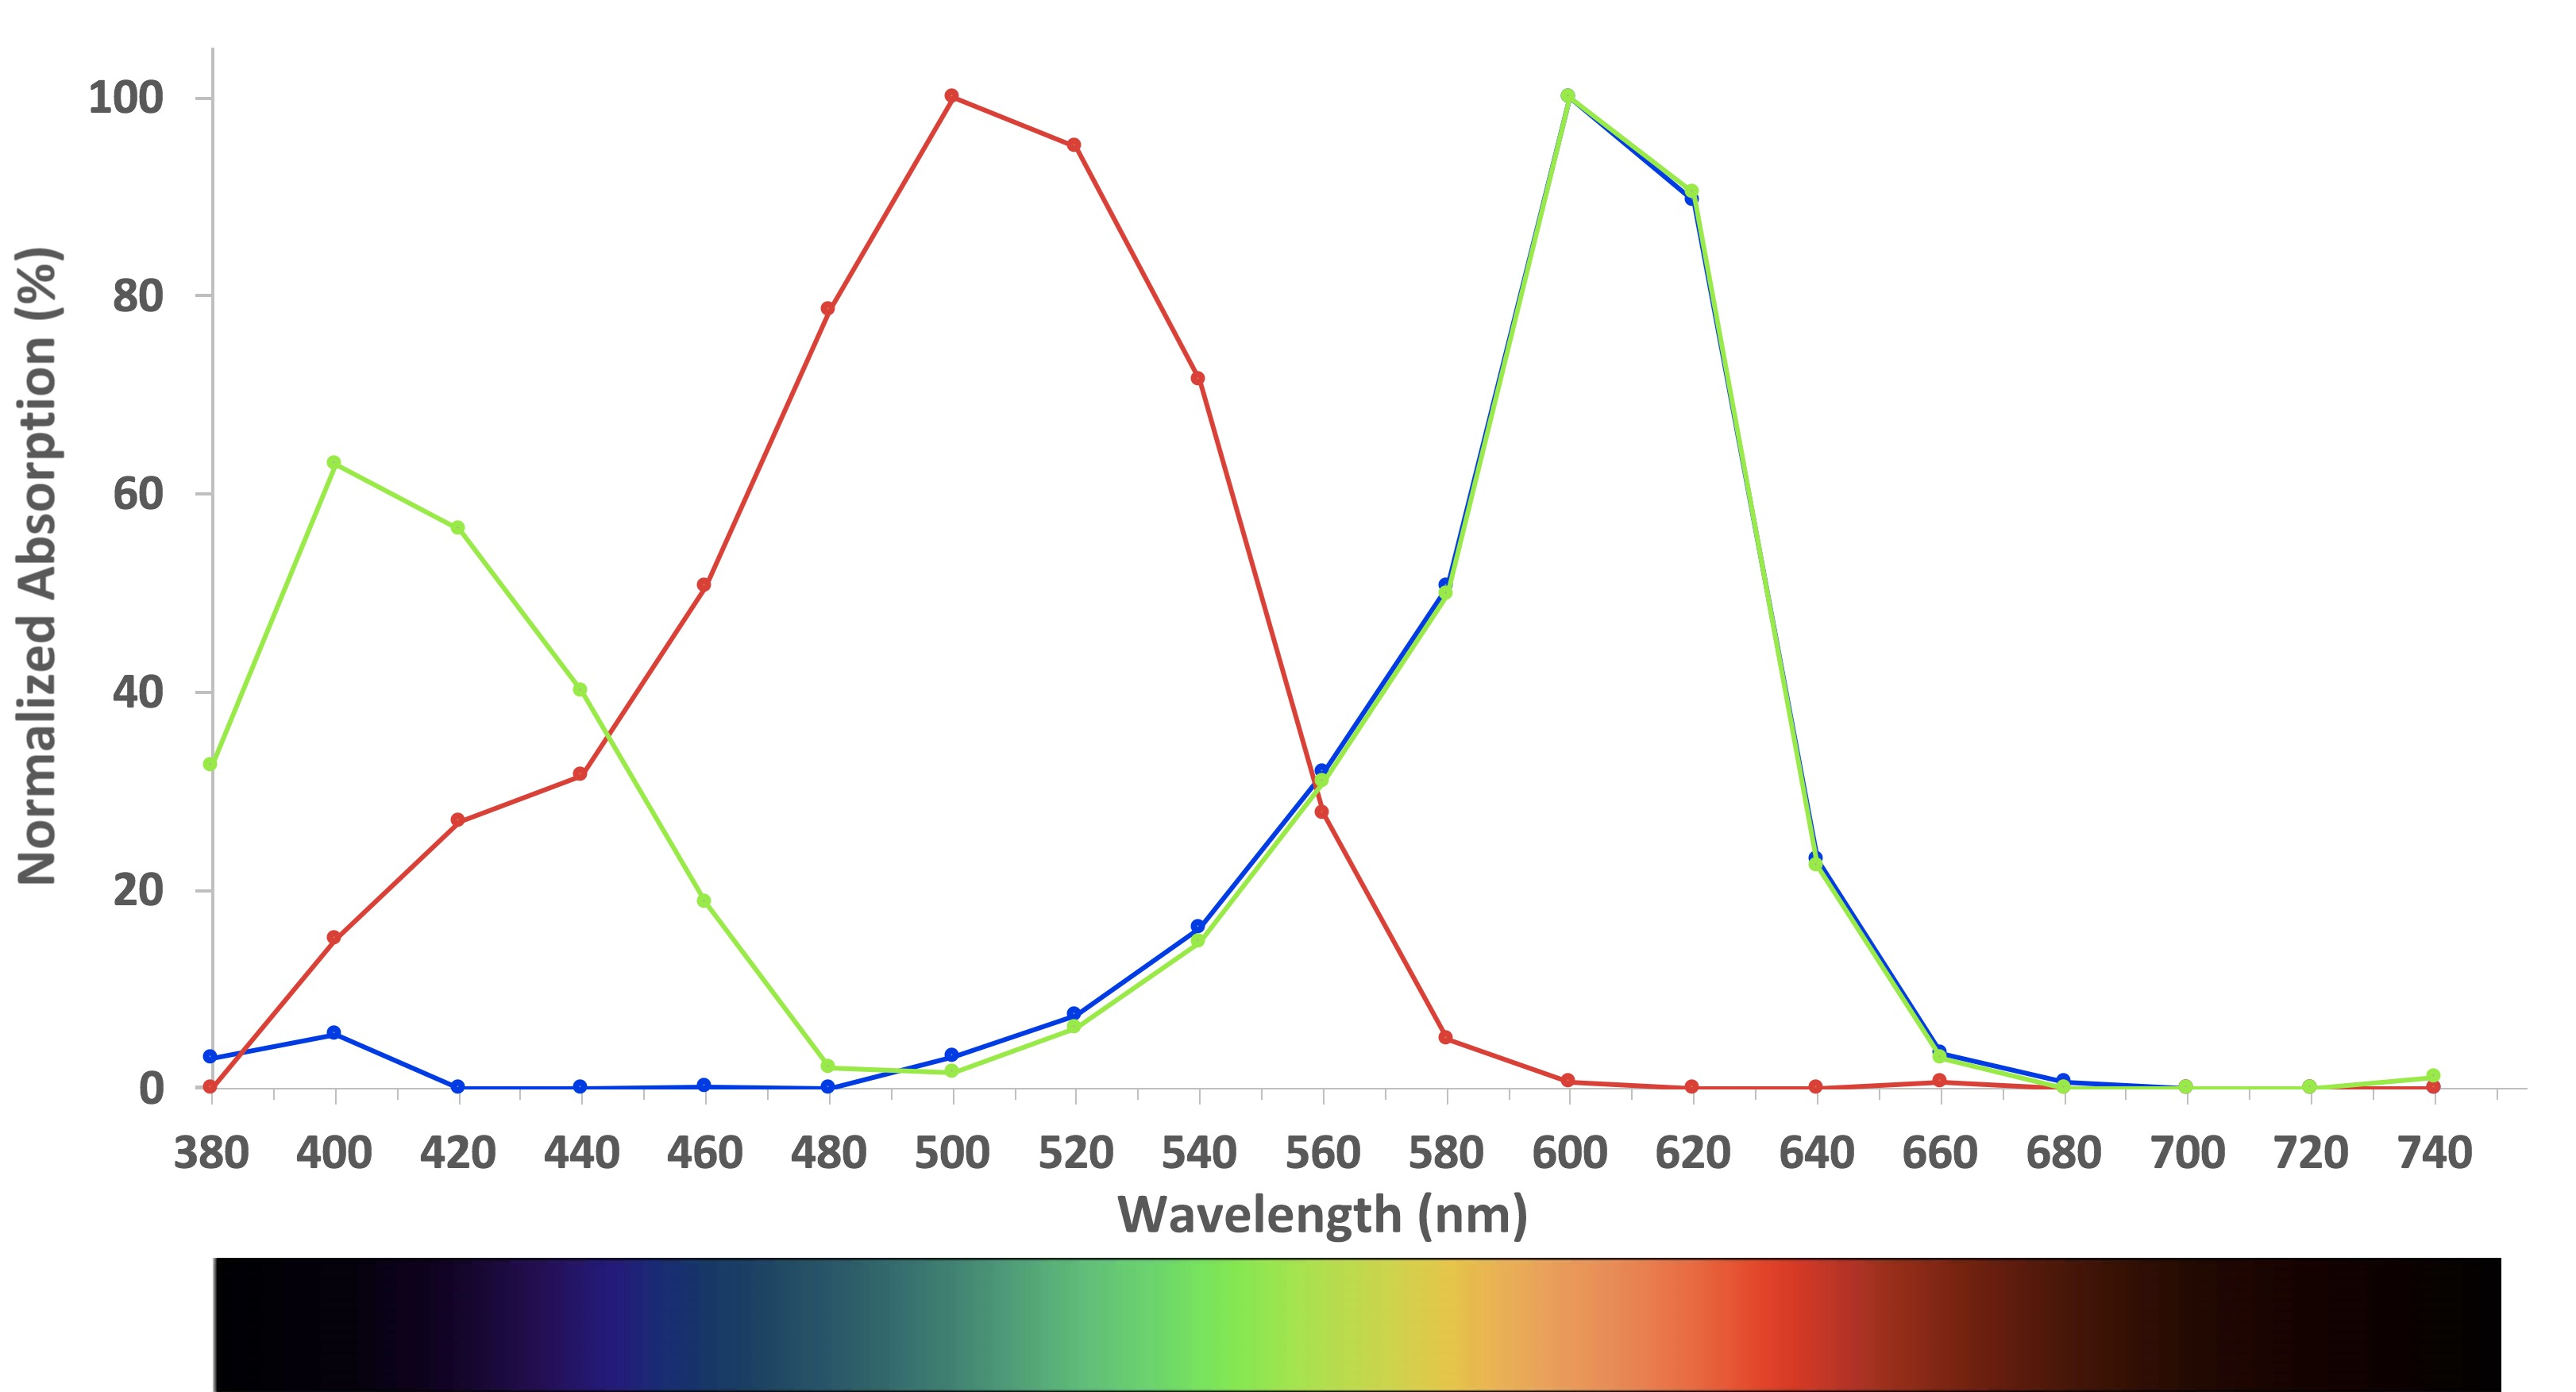
\includegraphics[width=0.7\linewidth]{./figures/photosynthesis/absorption_result}

}

\caption{Normalized absorption of red, green and blue dye solutions. Compare these data with your own results.}\label{fig:absorption}
\end{figure}

\section{Chromatography}\label{chromatography}

\href{https://en.wikipedia.org/wiki/Chromatography}{Chromatography} is a
laboratory technique for the separation of a mixture. The mixture is
dissolved in a fluid called the mobile phase, which carries it through a
structure holding another material called the stationary phase. The
various constituents of the mixture travel at different speeds, causing
them to separate. The separation is based on differential partitioning
between the mobile and stationary phases. Subtle differences in a
compound's partition coefficient result in differential retention on the
stationary phase and thus affect the separation. Chromatography may be
preparative or analytical. The purpose of preparative chromatography is
to separate the components of a mixture for later use and is thus a form
of purification. Analytical chromatography is done normally with smaller
amounts of material and is for establishing the presence or measuring
the relative proportions of analytes in a mixture.

In this experiment, we separate a mixture of food dyes (dark greenish
liquid. The mobile phase (separation buffer) is 1\% NaCl in water, the
stationary phase is chromatography paper.

\subsection{Experimental procedures}\label{experimental-procedures-27}

\begin{enumerate}
\def\labelenumi{\arabic{enumi}.}
\tightlist
\item
  Obtain a small beaker.
\item
  Add NaCl running buffer to the beaker until it reaches a height of
  about 5 mm.
\item
  Obtain a strip of chromatography paper and put it down on the bench.
\item
  Obtain the bottle containing the dark green food dye mixture.
\item
  Obtain a glass capillary and insert the tip of the capillary into the
  food dye mixture liquid. A little bit of dye will ascend into the
  capillary.
\item
  Remove the capillary and apply.
\item
  Touch the left side of the chromatography paper about 1 cm above its
  lower end with the tip of the capillary. A little bit of green liquid
  will spread out on the paper. Lift the capillary and touch the paper
  again just to the right of the dye you just applied. Repeat this until
  you have a horizontal line of dye from the left to the right side of
  the paper.
\item
  Place the chromatography paper into the beaker as shown below.
\item
  Observe how the running buffer moves up the paper and separates the
  dye mixture into three components (red, yellow and blue.
\end{enumerate}

\begin{figure}

{\centering 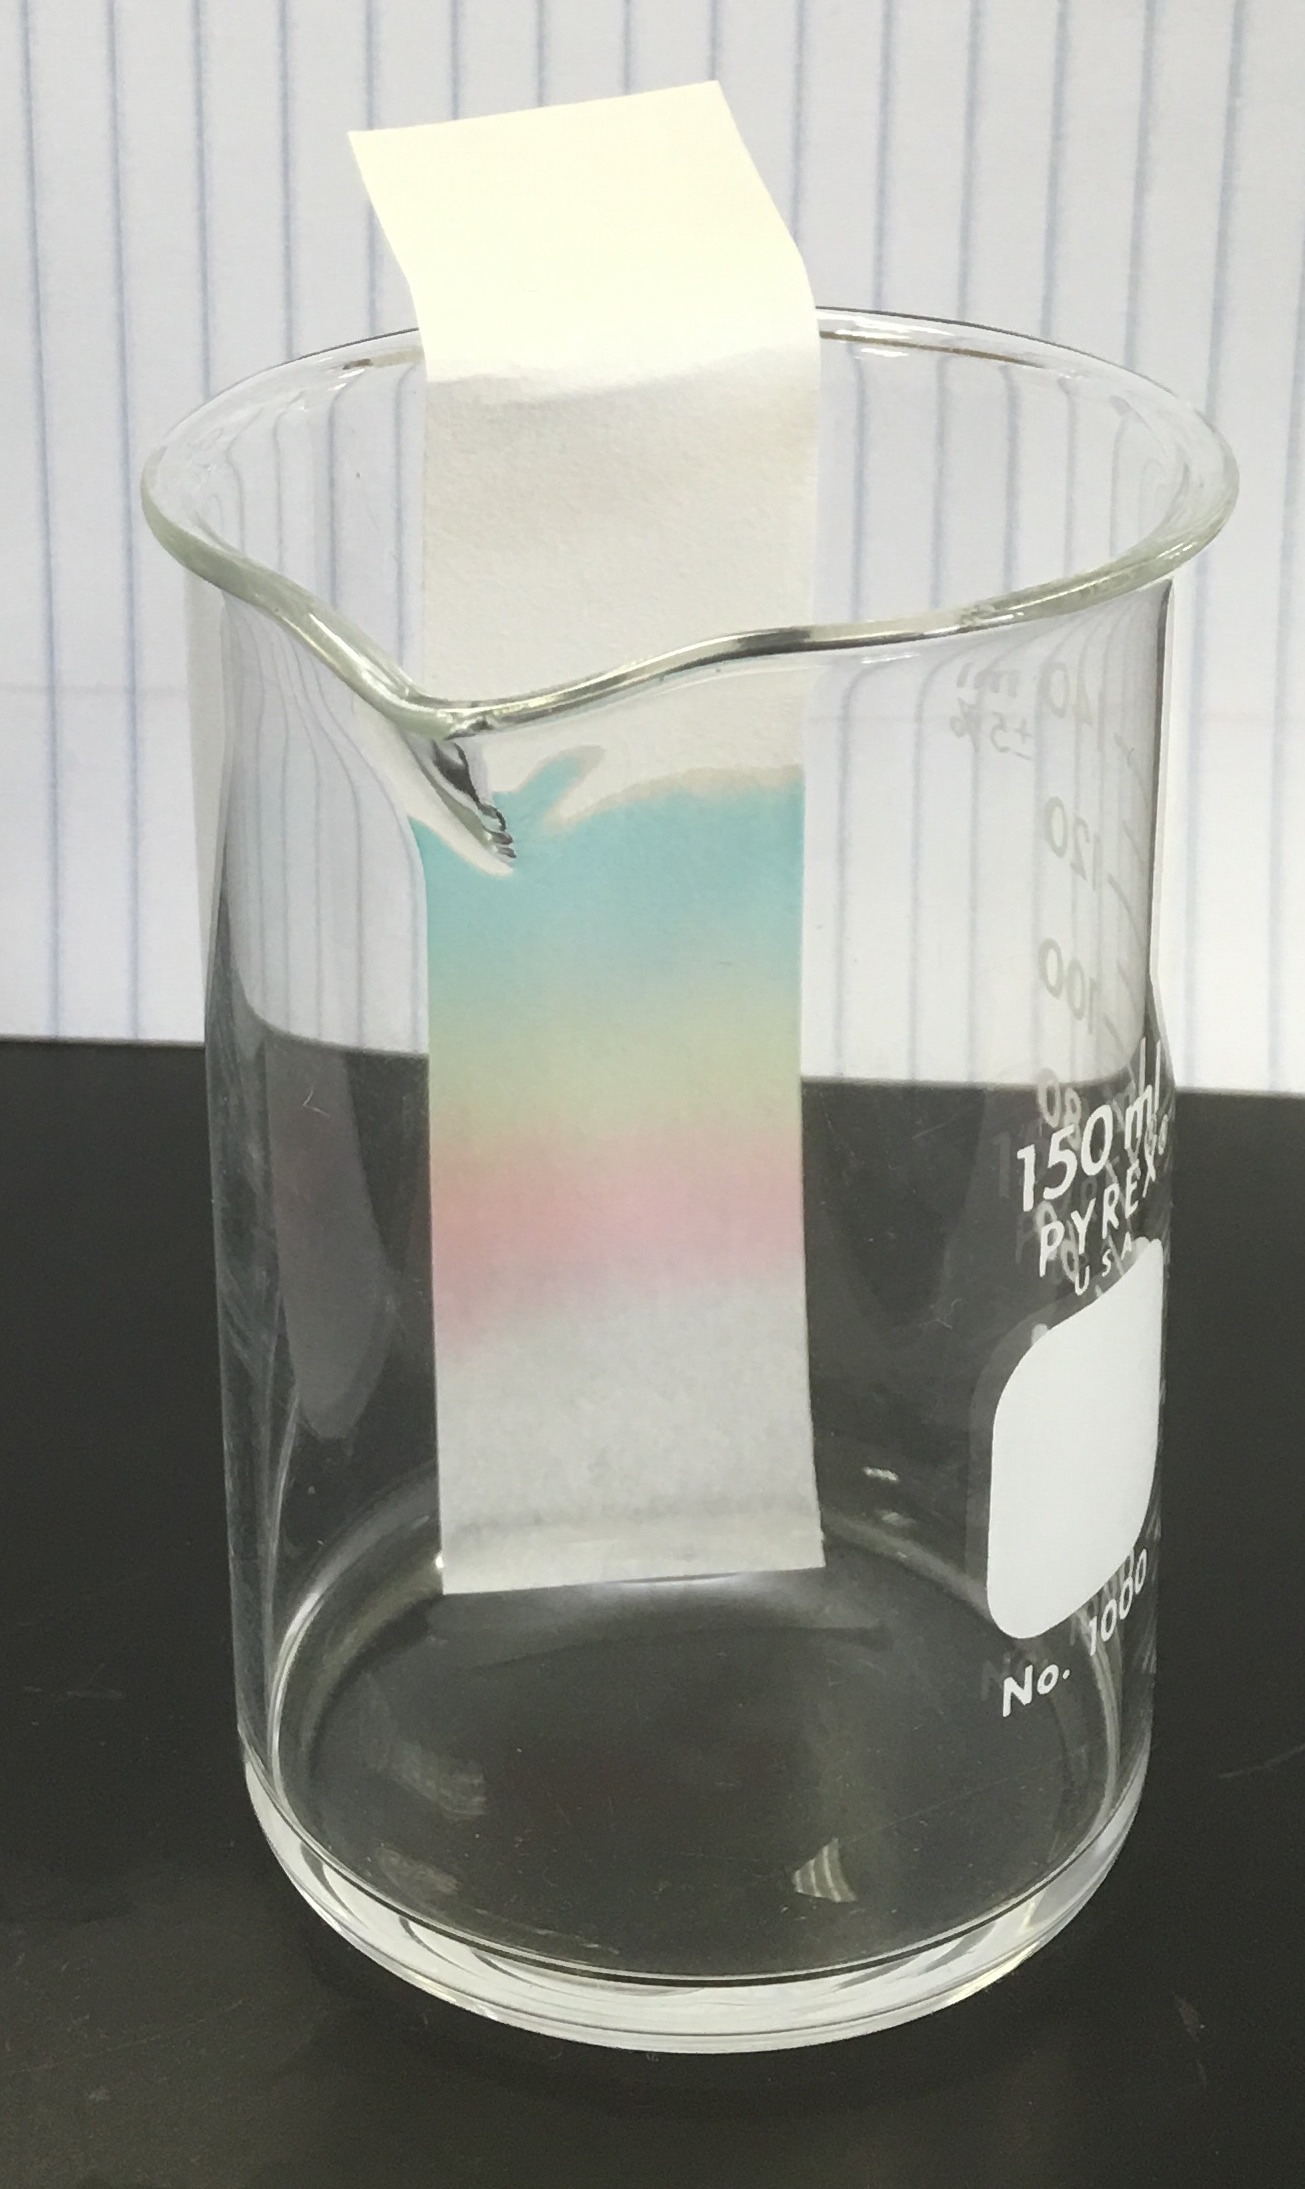
\includegraphics[width=0.7\linewidth]{./figures/photosynthesis/chromatography}

}

\caption{Result of the Chromatography experiment.}\label{fig:chromatography}
\end{figure}

\section{Review Questions}\label{review-questions-5}

\begin{enumerate}
\def\labelenumi{\arabic{enumi}.}
\tightlist
\item
  What is light?
\item
  In your own words, describe the endproducts of photosynthesis.
\item
  In your own words, describe what happens in photosynthesis.
\item
  What is chlorophyll and what does it do?
\item
  Where inside of plant cells does photosynthesis happen?
\item
  What is chromatography and what is it used for?
\end{enumerate}
